\clearpage
\section{Time-varying functional connectivity (TVFC)}\label{sec:tvfc}
%%%%%

\info[inline]{Paragraph: Introduce concept of time-varying functional connectivity.}
Is it fair to assume that \gls{fc} is temporally stable and stationary (i.e.~\emph{static}) across a measurement period?
In fact, many studies have shown that such connectivity varies across the length of a brain scan~\parencite{Chang2010, Sakoglu2010, Cribben2012, Lang2012, Hutchison2013, Hutchison2013b, Allen2014, Lindquist2014, Gonzalez-Castillo2015, Leonardi2015, Liegeois2017, Preti2017}.
Therefore, there is a growing interest in studying the time-varying nature of the functional relationship between brain regions.
Extending our estimation of \gls{fc} from \gls{sfc} to \gls{tvfc}, \textcite{Calhoun2014} proposed to call this functional connectome a `chronnectome', to avoid confusing it with the static (i.e.~scan average) analysis of \gls{bold} signal coupling.
%
Intuitively, it makes sense that, unlike anatomical connections, functional connections are likely to change in the timescale of a brain scan.
If brain region covariance structure is informative of cognitive processes, a change in task or mental occupation in a scanner should affect such structure.
And indeed, it has been shown to do so~\parencite{Doucet2012}.
%
\gls{tvfc} has quickly emerged as a popular topic of study in the field.
Several review papers have been written about it already~\parencite{Hutchison2013, Calhoun2014, Chen2017, Preti2017, Lurie2020}.
Most \gls{tvfc} research has been focused on \gls{rs-fmri} so far.\footnote{Before the rise of \gls{tvfc} studies, \gls{sfc} was often simply referred to as `resting-state functional connectivity' (RSFC or rsFC).}
A typical \gls{tvfc} workflow is shown in \cref{fig:tvfc-workflow}.


\begin{figure}[t]
  \centering
  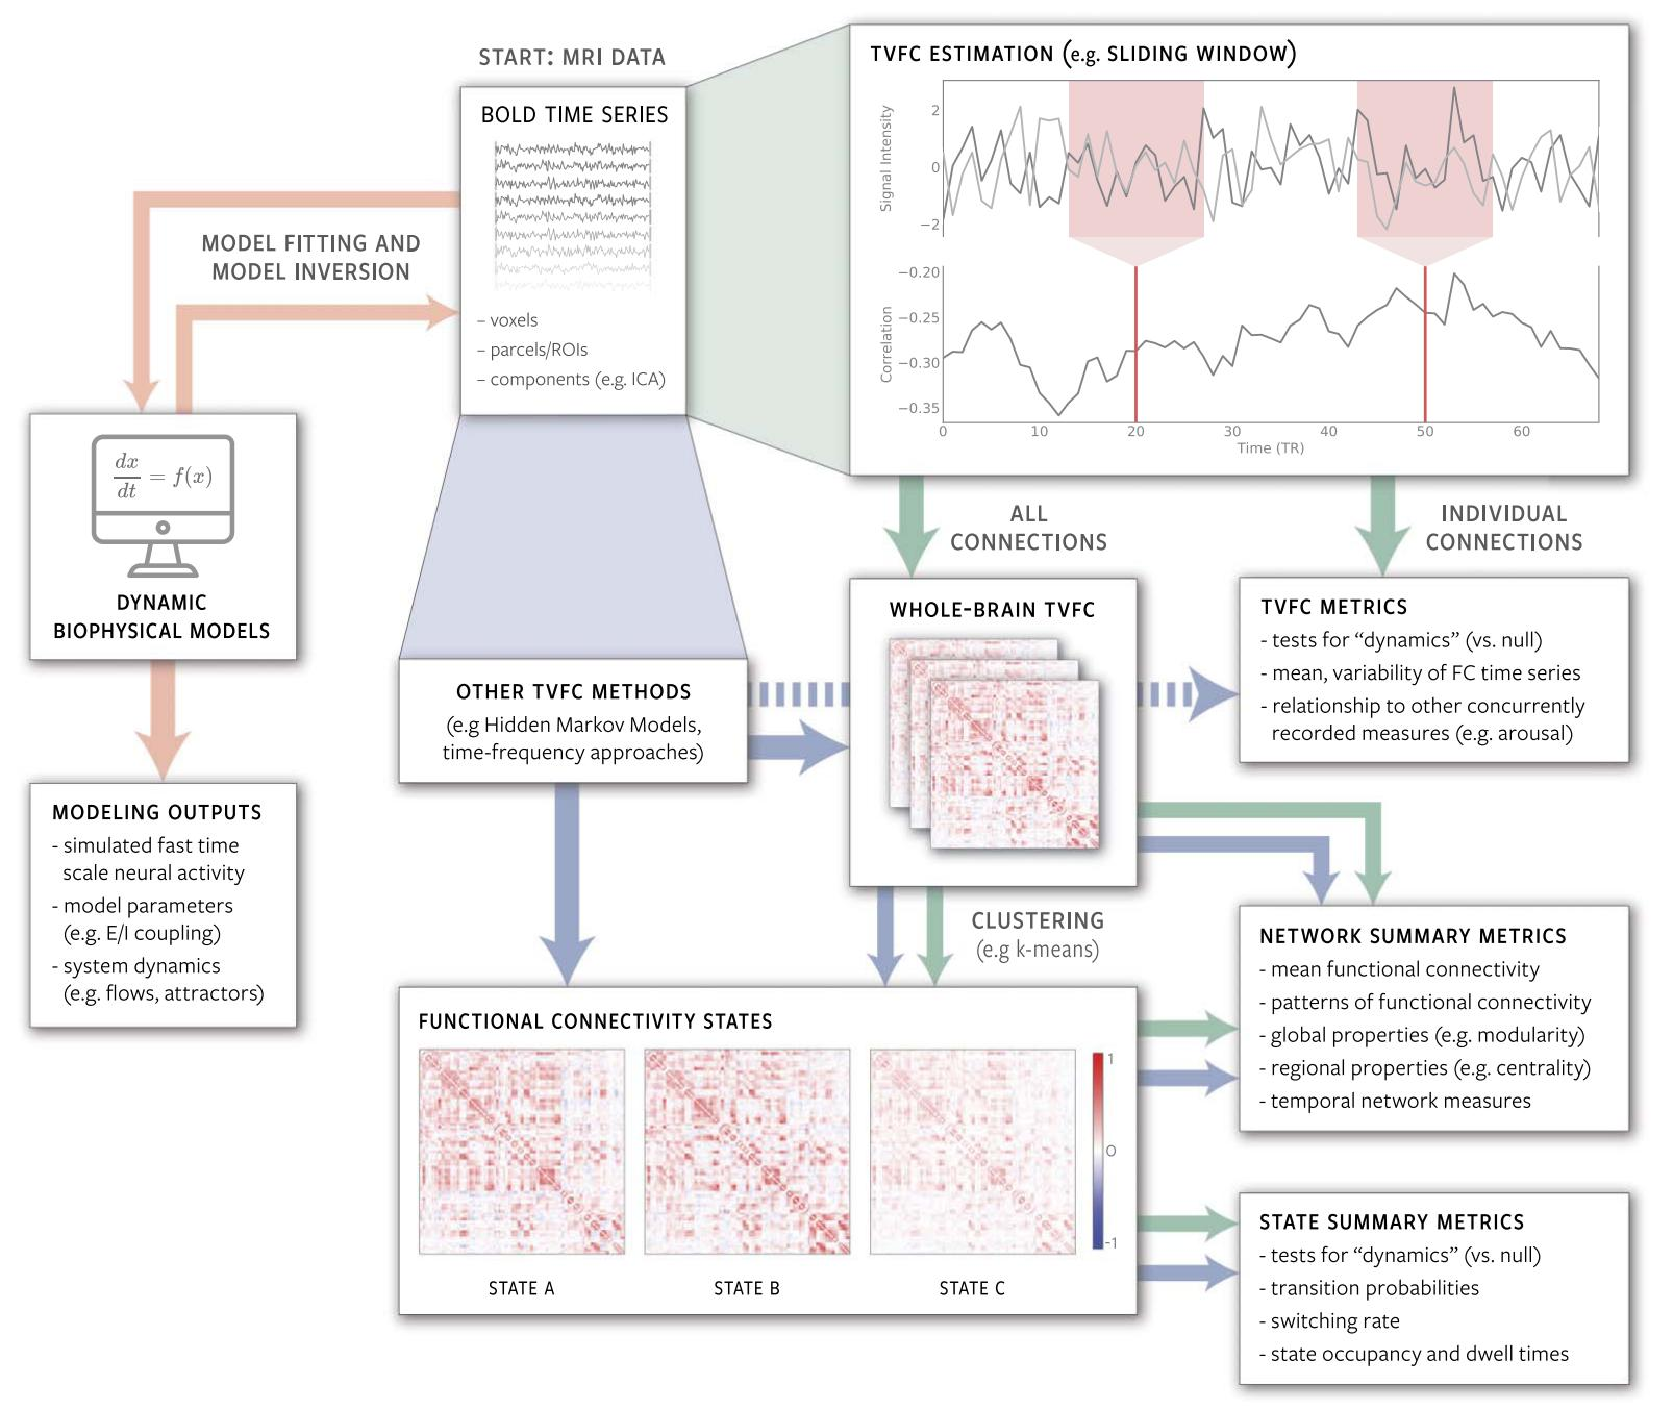
\includegraphics[width=\textwidth]{fig/tvfc_methods_Lurie2020_compressed}
  \caption{
    Typical TVFC estimation and feature extraction workflow(s) in fMRI data.
    Green arrows show a typical sliding-windows analysis, blue arrows indicate a range of other data-driven analyses, orange arrows represent fitting a biophysical model to time series data.
    Re-generated from \textcite{Lurie2020}.
  }\label{fig:tvfc-workflow}
\end{figure}


\info[inline]{Paragraph: Clear up TVFC naming convention.}
Before moving on, we need to address some housekeeping regarding naming conventions.
The terms \gls{tvfc} and \gls{dfc} (or dynFC) are sometimes used interchangeably, but sometimes refer to different things.
To avoid confusion, we will use the more general term \gls{tvfc} and a broad label, since `dynamic' functional connectivity is used in multiple ways and contexts across disciplines~\parencite[see][for more details]{Lurie2020}.

\info[inline]{Paragraph: Discuss scientific insights from TVFC.}
Although \gls{sfc} analyses have taught us a lot, \gls{tvfc} can increase our understanding of the underlying cognitive processes that generate such covariance structures~\parencite{Cohen2018}.
The study of \gls{tvfc} can help the understanding of adaptation and shifts in behavior in the brain.
%
Since \gls{tvfc} is an extension of \gls{sfc}, all information captured by \gls{sfc} should be captured by \gls{tvfc} too.
Therefore, we argue that \gls{tvfc} should always be compared to \gls{sfc} to find out what extra information is extracted from including the time-varying nature of the covariance structure.
And indeed, \gls{tvfc} has been shown to extract additional information in some cases compared to just \gls{sfc}~\parencite[see e.g.][]{Rashid2016, Jin2017, Liegeois2019, Luppi2019, Varley2020, Vidaurre2021, Coppola2022}.
These results also suggest that the study of consciousness and certain mental disorders may benefit from a dynamic view of the brain.
%
Despite these insights, there are still many open questions regarding the interpretation and validity of \gls{tvfc} estimates.
The biological and physiological basis of \gls{tvfc}, both neural and nonneural in origin, is still elusive~\parencite{Lurie2020}.
\textcite{Liu2013, Petridou2013} have suggested that \gls{tvfc} may originate from transient coactivation patterns (CAPs) and their dynamics.
\textcite{Matsui2019} later confirmed this by simultaneously recording calcium imaging and optical hemodynamics~\parencite[see][for a review of multi-modal approaches]{Thompson2018b}.
Furthermore, it has often been suggested that the brain exhibits a state-space structure, which may underlie the observed time-varying connectivity structure~\parencite{Hutchison2013}.
Such `brain state' characterizations entail the evolving dynamics and self-organization of brain networks~\parencite{Kringelbach2020}.
The particular definition in our \gls{fmri} \gls{fc} context will be discussed more in \cref{subsec:brain-states}.

\info[inline]{Paragraph: Discuss open questions and limitations.}
There are ongoing debates about the physiological origins and relevance (behaviorally as well as cognitively) of \gls{tvfc}.
\textcite{Laumann2017} challenged the idea that \gls{tvfc} is related to ongoing cognition.
One potentially compelling argument against any cognitive relevance of \gls{tvfc} is that \gls{fc} fluctuations have also been observed in anesthetized (unconscious) brains~\parencite{Hutchison2013b}.
However, \textcite{Demertzi2019} found anesthesia to change network complexity, validating its implication with consciousness~\parencite[see also][]{Varley2020b}.
Furthermore, questions have been raised about the statistical validity of this construct.
As \textcite{Lurie2020} discussed, fluctuations and correlations may well be explained by nonneural physiological factors such as head motion, cardiovascular, and respiratory effects.
%
It is critical that these ambiguities are resolved before we make inferences in high-stakes settings, such as when studying mental disorders.
The work in this thesis aims to help clarify and resolve such issues.
